\subsection*{Add.2}
\paragraph{}
The scalarized problem is clear a GP since it can be written as the following form
\begin{align*}
&\text{minimize} \qquad \sum_{i=1}^6w_i + ut \\
&\text{subject to} \quad \ \  w_i - w_{max} + 1 \leq 1 \qquad i=1,...,6\\
& \qquad \qquad \qquad  w_{min} - w_i + 1 \leq 1 \qquad i=1,...,6\\ 
& \qquad \qquad \qquad  T_i - t + 1 \leq 1, \qquad i=1,...,3
\end{align*}
\paragraph{}
Where the objective function and constraints are posinomials.
\begin{figure}
	\centering
	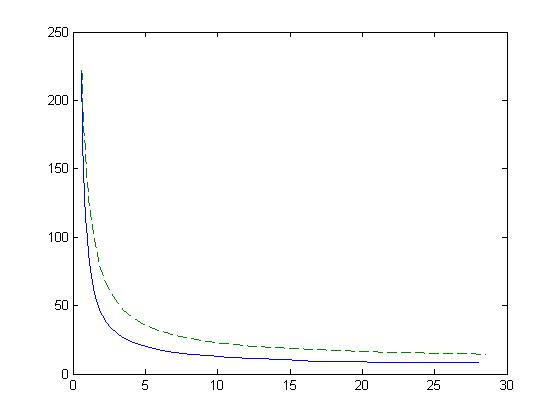
\includegraphics[scale=0.7]{Compare.jpg}
	\caption{Comparison}
\end{figure}
\paragraph{}
\verbatiminput{ic_main.m}
